\section{Realtime Compilation for Continuous Angle Rotation Architectures}
In this section, we discuss the compilation of high level programs to surface code architectures which support Clifford+Rz gates as opposed to the traditional Clifford+T. We assume all programs have already been synthesized into the appropriate gate set. In typical distillation architectures, factories are bulky and hard to intersperse amongst the data qubits. Therefore, resource states are prepared and stored remotely on the boundaries, only to be routed in for consumption as necessary. In contrast, in small angle rotation architectures, only small seeds of $\ket{m_{\theta}}$ states are prepared and expanded locally into surface code qubits. It takes at most a single logical patch for preparation at the cost of additional uncertainty in its preparation time. In prior work, atomic units of data qubits and ancilla for the preparation of single qubit gates are prepared. We, however, propose a much more flexible architecture which allows ancilla to be reused and allocated for various rotations dynamically.

\subsection{Execution of \texorpdfstring{$Rz(\theta)$}{Rz(theta)} Rotation Gate}
As discussed in Section~\ref{section:relatedwork}, the $Rz(\theta)$ rotation gate is executed in two steps, a. preparation of an ancilla qubit in the state $\ket{m_\theta}$, and b. injection of the $\ket{m_\theta}$ state into the data qubit and measurement. If the measurement output signifies a failure (with probability $1/2$), a correction $Rz(2\theta)$ would be required. If this correction fails, another correction gate $Rz(4\theta)$ would be required and so on, in a Repeat-Until-Success (RUS) manner. Specifically, failed injection means a $Rz(-\theta)$ was prepared so a $Rz(2\theta)$ correction would yield the proper rotation. However, since $Rz(2\theta)$ is likely a non-Clifford we must repeat. In general, if an $Rz(2^k\theta)$ injection fails we require $Rz(2^{k+1}\theta)$ correction. Every injection fails with probability $1/2$, hence
\begin{align*}
\mathbb{E}[\text{Num. Injections}] &= \sum_{k=1}^{\infty} k \cdot \text{Pr[k-1 Failures, 1 Success]} \\
&= \sum_{k=1}^{\infty} \frac{k}{2^k} = 2
\end{align*}

\begin{figure}
    \centering
    \begin{quantikz}[transparent]
                                            & \gate[wires=5]{M_{P\otimes Z}}  & \gate[wires=4]{P} & \qw\\
                                            &                                 &                   & \qw\\
                                            &                                 &                   & \qw\\
                                            &                                 &                   & \qw\\
    \lstick{$\overline{\ket{m_\theta}}$}    &                                 & \meterD{M_X}\vcw{-1}
\end{quantikz}
    \caption{A Pauli-product measurement circuit}
    \label{fig:pauliprod}
\end{figure}
\begin{figure}
    \centering
    \begin{quantikz}[transparent]
    \lstick{$\overline{\ket{\psi}}$}        & \targ{} & \gate{X} & \rstick{$Rz(\pm\theta)\overline{\ket{\psi}}$}\\
    \lstick{$\overline{\ket{m_\theta}}$}    & \ctrl{-1} & \meterD{M_Z}\vcw{-1}
\end{quantikz}
    \caption{A Rotation gate injection circuit}
    \label{fig:rzrotation}
\end{figure}
\begin{table}
    \centering
    \begin{tabular}{|c|c|c|}
        \hline
        Parameter & CNOT & ZZ \\
        \hline
        Exposed edge & X & Z \\
        Number of ancillas required & 2 & 1 \\
        Lattice surgery cycles needed for injection & 2 & 1 \\ % TODO: @Jonathan please confirm this again
        \hline
    \end{tabular}
    \caption{Difference between the two injection strategies}
    \label{table:LvsZZ}
\end{table}
In the case where $Rz(2^k\theta)$ is a Clifford for some $k$ (for example consider T or $\sqrt{T}$), this expectation will be $< 2$ since it will no longer require an injection step. There are two potential strategies for injection, summarized in Table~\ref{table:LvsZZ}, one using a CNOT (Figure~\ref{fig:rzrotation}) and one using a ZZ pauli-product measurement (Figure~\ref{fig:pauliprod} with $P = Z$). In either case, the compiler must allocate a contiguous block of ancilla. Our compiler reserves ancilla and generates a schedule for each ancilla (either dynamically or statically) determining when its free; we simply require that some path between $\ket{m_\theta}$ and target all be free at some time.

The preparation of the rotation states $\ket{m_\theta}$ is itself non-deterministic and is prepared in an ancilla patch. Consequently, assigned ancilla are claimed for an indeterminate number of cycles until the state is prepared correctly. Different states $\ket{m_\alpha}$ and $\ket{m_\beta}$ require disjoint ancilla for preparation. Multiple ancilla can be assigned for the preparation of any individual state and any additional successful preparations can be discarded if necessary. The number of ancilla dedicated to the production of a particular state $\ket{m_\theta}$ can dynamically change; for example if $n$ ancilla are assigned in cycle 1 and each fails and some $m$ of these ancilla are needed for other operations, we can reclaim them and in the next cycle try to prepare the state using $n - m > 0$ ancilla. Non-deterministic preparation implies that the exact cycle when consumption can occur is unknown a head of time and motivates eager preparation.

Thus, any compilation strategy would need to consider which ancillas are good candidates for the preparation (and injection). Additionally, the compiler would need to decide when the preparation starts. Starting the preparation too early would end up hogging resources for another gate operation, since the prepared ancilla is not freed until the injection completes. On the other hand, preparing too late would lead to slower execution of the rotation gate since the data qubit would be waiting on the preparing ancilla. In an ideal scenario, the preparation should begin so that the ancilla is prepared exactly when the data qubit becomes available for the injection.


\subsection{Execution of CNOT Gate}
% routing and rotation
Lattice surgery on surface codes gives us a convenient way to perform CNOT gates between two data qubits that can be arbitrarily far apart in constant time (taking $2$ lattice surgery cycles). The only requirements for the execution is that there should exist a path of ancilla qubits connecting the control to the target (via at least one ancilla qubit), and the path should be from the Z edge of the control qubit to the X edge of the target qubit. It might be possible that such a path does not exist, either due to the ancillas being occupied for another gate operation, or the required edges (X or Z edges) of the data qubit not having any neighboring ancillas (see Section~\ref{section:variableancilla} for an example of this situation). In such cases, the compiler would need to insert an edge-rotation gate to orient the correct edge of the qubit onto the chosen path. This gate operation requires one free ancilla qubit and takes $3$ lattice surgery cycles.\par
The quality and speed of the algorithm used for path computation is thus an essential consideration for the compilation strategy. The compiler should also be able to insert the edge-rotation gates as and when required, while also minimizing the need for the edge-rotation gates. For example, Figure~\ref{fig:cnot_selection} shows two different selection algorithms. Both algorithms choose the \textit{shortest} path, however the naive selection of shortest may potentially lead to selecting an ancilla that is being used by a lot of other gate operations and this might lead to delayed start of the CNOT execution since the ancilla might not be free until much later.
\begin{figure}
    \centering
    \begin{subfigure}{0.49\columnwidth}
        \includesvg[width=\linewidth]{figs/cnot_selection_1.svg}
        \caption{Shortest path}
    \end{subfigure}
    \begin{subfigure}{0.49\columnwidth}
        \includesvg[width=\linewidth]{figs/cnot_selection_2.svg}
        \caption{Path with earliest start time}
    \end{subfigure}
    \caption{Different CNOT routing strategies between the two gray data qubits. The darkness of the ancilla qubit indicates the activity of the ancilla.}
    \label{fig:cnot_selection}
\end{figure}

\subsection{Variable Ancilla Availability}\label{section:variableancilla}
% sharing of ancillas across patches
A flexible architecture is considered with a fraction of the data qubits residing in a \textit{compact patch} and the other fraction of the data qubits make up the \textit{regular patch}. Such an architecture also motivates the need to share the ancillas between the qubit patches due to limited resources available to each patch by itself. This allows for better consideration of an actual system with finite resources and non-uniform resource allocation. The compiler needs to take the locally available and shared resources into account when determining which ancillas to use for different operations and how to maximize parallel computation.

\subsection{Static Compilation for Continuous Angle Rotation Architectures}
% the static compilation strategy
\begin{figure}
    \centering
    \scalebox{0.7}{
    \begin{quantikz}[transparent]
    \lstick{$\ket{q_1}$} & \ctrl{6} & & \gate{Rz(\theta_1)} & \qw\\
    \lstick{$\ket{q_3}$} & & \ctrl{2} & & \qw\\
    \lstick{$\ket{q_5}$} & & & \ctrl{3} & \qw\\
    \lstick{$\ket{q_6}$} & & \targ{} & & \qw\\
    \lstick{$\ket{q_7}$} & & \gate{Rz(\theta_7)}\slice{} & & \qw\\
    \lstick{$\ket{q_8}$} & & & \targ{} & \qw\\
    \lstick{$\ket{q_9}$} & \targ{} & & & \qw
\end{quantikz}}
    \caption{Example circuit for execution of the static compiler shown in Figure~\ref{fig:baseline_execution}}
    \label{fig:baseline_circuit}
\end{figure}
\begin{figure*}
    \centering
    \includesvg[width=\textwidth]{figs/baseline_execution.svg}
    \caption{Execution begins at time $t_1$. For layer 1, the ancillas being used for CNOT between $q_1$ and $q_9$ are colored in orange, CNOT between $q_3$ and $q_6$ are colored in yellow, and $Rz$ on $q_7$ are colored in red. Note that the CNOT between $q_3$ and $q_6$ requires to edge-rotate $q_6$ to orient the edges correctly. Completion of the gate execution is indicated by the ancillas turning green. For layer 2, the ancillas being used for the CNOT between $q_5$ and $q_8$ are colored in orange and the $Rz$ on $q_1$ are colored in red.}
    \label{fig:baseline_execution}
\end{figure*}

We consider a static compilation strategy that divides the circuit into layers of gates that can be executed in parallel. The input circuit is divided into layers by iterating on the gates in the order of execution and reserving the ancillas for exactly one gate operation per layer. If a particular gate cannot be executed in the current layer because of lack of ancilla resources, the compiler attempts to execute the gate in the next layer.\par
For the $Rz(\theta)$ gates, we only consider a single ancilla qubit for the preparation, depending on the patch configuration and the exposed edges. For the execution of CNOT gates, the shortest path between the control and target is chosen. While computing the shortest path, only the ancillas that have not been reserved for the current layer are considered. If the need for an edge-rotation is found for the chosen path, edge-rotation gates are inserted before and after the CNOT gate. The rotation gates are inserted after the CNOT gate to ensure that the correct edges continue to remain exposed for the $Rz(\theta)$ gate injection. Choosing the shortest path helps to maximize the parallelism in each layer since the next gate has more ancillas available to choose from. If the control and target cannot be connected, then gate is skipped in the current layer. Figure~\ref{fig:baseline_execution} shows an example execution for the circuit shown in Figure~\ref{fig:baseline_circuit}.

\section{Dynamic Compilation}
In this section, we discuss our dynamic compilation strategy that aims to minimize the total program execution time by executing the gate operations as soon as possible. The performance improvements of this strategy are based on two major observations:
\begin{enumerate}
    \item Multiple ancillas can be prepared in parallel and the preparation can begin before the actual $Rz(\theta)$ gate operation can begin.
    \item The expected `free' time of the ancilla qubits, that is, the time when the ancilla qubits are going to be available for connecting the control and the target, can be used to make instantaneous decisions when determining the best path for the CNOT gate execution
\end{enumerate}
The first observation motivates the need to efficiently manage and allocate the ancillas available to the different gates and data qubits. Since the preparation and injection for the $Rz(\theta)$ rotation gates is done locally, it makes the management feasible with a negligible classical overhead and thus it can be done during runtime without any performance penalty. The exact techniques used are discussed in Section~\ref{section:ancillamanage}.\par
Finding the best path in a graph (the 2D grid of the data qubits and ancillas) such that it can begin execution at the earliest is equivalent to solving the minimax path in a graph. This problem has a polynomial time solution which is obtained by computing the Minimum Spanning Tree and connecting the control and target on this tree. However, the complexity of this algorithm is $O((N + E)\log{E})$ where $N$ is the number of logical qubits in the grid and $E$ is the number of edges. Since we are considering a 2D grid, $E = O(N)$ and therefore the time complexity can simply be written as $O(N\log{N})$. Thus this approach would scale with the size of the grid and would be inefficient. Indeed, if we consider a classical computation unit that runs at $2$ GHz and assume that we require about $10N\log{N}$ instructions to compute the MST, for a quantum system with $100$ data qubits, it would require between 1-2$\mu s$ to compute the MST for a single CNOT gate. These calculations have been done assuming an IPC (instructions per cycle) of $1$, however, in reality, the IPC of any system is much lower and hence the number of cycles required would increase significantly. Therefore, this leads to a huge overhead and we cannot always choose the best path without introducing huge stalls for each CNOT execution. Instead we propose a strategy that uses the second observation and computes a single tree every $k$ cycles, thus making the computation efficient while also maintaining knowledge of the recent occupancy of the ancilla qubits. We discuss this approach in detail in Section~\ref{section:efficientmst}

\subsection{Intelligent Ancilla Resource Management}\label{section:ancillamanage}
\begin{figure*}
    \centering
    \includesvg[width=\textwidth]{figs/prepare_timeline.svg}
    \caption{An example execution for an $Rz(\theta)$ gate to be executed next on the middle data qubit. The qubit in grey is another data qubit. Time steps $t_1$ and $t_2$ show execution times when different sets of ancilla qubits are busy. $T_i = t_3$ is when it is determined that the data qubit would be free at time $T_d = t_5$ and thus we start preparing all possible ancilla qubits in the neighborhood. Another ancilla qubit becomes free at time $T_a = t_4$ and we start preparing it. At $t_6$, one ancilla qubit succeeds in preparation and thus the injection begins, simultaneously we start preparing ancillas in the state $\ket{m_{2\theta}}$. The injection completes at time $t_7$ and $\ket{\psi'} = Rz(-\theta)\ket{\psi}$, thus we need to perform the correction gate.}
    \label{fig:prepare_timeline}
\end{figure*}

The execution of any gate can be broadly broken down into two steps, preparation and execution. The preparation step only requires the associated ancilla qubits to be free while the execution step requires the data qubit(s), prepared ancilla qubit(s) and any ancilla qubit connecting these qubits to be free. Thus, if we consider the timeline of execution of the gate, the preparation can be done asynchronously. The execution step may or may not require more ancillas apart from the ancilla that was used in the preparation step. Also some gates might not have any preparation step at all.\par
This is especially important for the dynamic compilation of the $Rz(\theta)$ rotation gates. Consider a single ancilla qubit being used for the preparation of the $Rz(\theta)$ gate. For the ancilla and data qubits, we define the parameters $t_\theta$, $T_d$, $T_a$, $T_b$, $T_i$ to understand the dynamic compilation step. $t_\theta$ is the expected time it takes to prepare the ancilla qubit in the state $\ket{m_\theta}$. The time when the data qubit is free and can participate in the execution of the gate operation is denoted by $T_d$. Similarly, the time when the ancilla qubit is free and it can participate in the preparation of the gate operation is denoted by $T_a$. In an ideal scenario, we would want to begin the preparation of the ancilla qubit at time $T_b = \max\left(T_d - t_\theta, T_a\right)$. However this might not always be possible. To understand why, we also consider the time $T_i$. This is the time during the execution of the program when it can be deterministically asserted that the data qubit is going to be free at time $T_d$. This is important since it might be possible that the total execution time for the $Rz(\theta)$ gate is longer or shorter than the expected time. Let us consider the case when $T_a < T_d - t_\theta$. In this case, we would want to begin the preparation of the ancilla at $T_b = T_d - t_\theta$. However, if $T_i > T_b$, the compiler cannot physically determine that the data qubit can participate in the execution from time $T_d$ and thus it cannot actually begin the preparation until time $T_i$. Figure~\ref{fig:prepare_timeline} shows an example execution and relevant timestamps.\par
Another way to reduce the expected execution time of the $Rz(\theta)$ gates is by preparing multiple ancilla qubits in parallel. The more ancilla qubits that are prepared in parallel, the lesser the combined expected time of preparation is. We also permit sharing of the ancilla qubits between different data qubits. Additionally, the paths for connecting distant qubits for CNOT gates also passes through the patches of various data qubits. Therefore we need a dynamic ancilla allocation strategy that can determine when to assign which ancilla to which gate operation. Before we discuss the exact strategy, we note that the ancilla qubits used for the preparation and injection are only those that are present in a $3\times 3$ block with the data qubit in the centre. This is done to simplify the data structures that keep a track of the different ancilla qubits. Additionally, using the ancilla qubits that are far away would lead to making more global decisions and this would lead to increased resource contention since connecting the data qubit to the far away ancilla qubits would require freeing the ancilla qubits on the path.

\subsubsection{Queue for Ancillas}
To make it easy to keep a track of the gate operations that the ancilla qubits will assist, either during the preparation or during the execution, each ancilla qubit maintains a queue of the gate operations that the ancilla has prepare/execute for. The compiler then looks at the head of the queue and begins the required steps necessary for the gate operation. Similarly, when the compiler chooses the relevant ancilla qubits for a particular gate's operations, it pushes the gate to the queue of all the associated ancillas. As shown in Figure~\ref{fig:queue_timeline}, each queue entry needs to store some relevant information about the ancilla's role in the preparation and/or execution. In the case of a Rz gate, it might be possible that the ancilla is only being involved for execution, however, it might be associated with two different preparing ancillas as is the case for ancilla $3$. In such scenarios, it might be possible that the ancilla which is not the head of the queue gets prepared first. The compiler then removes all entries in queue that appear before this entry from the queue for this gate even if they appear in the middle of the queue. Most of the queue operations can be performed independently irrespective of the state of the queue of the other ancillas. Therefore, the queues for all ancillas can be maintained in parallel using small computation units for each ancilla with minimal support for coherence.

\begin{figure}
    \centering
    \includesvg[height=0.905\textheight]{figs/queue_timeline_vert.svg}
    \caption{Execution of the circuit with the queue. The text in bold signifies the current state of the ancilla. The dashed nodes represent the nodes that are being deleted from the queue.}
    \label{fig:queue_timeline}
\end{figure}

\subsection{Routing Strategy}\label{section:efficientmst}
\begin{figure}
    \centering
    \includesvg[width=\columnwidth]{figs/mst_selection.svg}
    \caption{Timeline showing the MST computation procedure. The MST computation begins at $t_1$ and the result is available by $t_2$. Another MST computation begins at $t_2$ and its result is available by $t_3$. For simplicity, here $k = p = t_2 - t_1 = t_3 - t_2$}
    \label{fig:mst_selection}
\end{figure}
Now that we have a convenient way to claim ancillas for the gate operations, all that remains is to efficiently determine the path of ancillas that will be used to execute any CNOT gate. To get an estimate of the activity of each ancilla during runtime, the MST algorithm is run on the sub-grid comprising of the ancilla qubits every $k$ cycles, where $k$ is a modifiable parameter. Assuming that the computation of the MST takes about $p$ cycles, the results of the MST computation are \textit{delayed} by $p$ cycles. If we use the weight of each ancilla during the MST computation as the expected time when the ancilla finishes execution, the information would be stale by the time the MST is computed. Thus, instead we use the expected activity of the ancilla in the last $p$ cycles to capture the \textit{heat} (activity) of each ancilla. Now when a CNOT gate requires to be executed, it just looks at the latest available MST and computes up to $4$ different paths. These paths computed are the paths from the $Z\to X$, $X\to Z$, $X\to X$, $Z\to Z$ edges of the control $\to$ target respectively. Note that all paths might not always exist. For the existing paths, the earliest expected start time is computed after accounting for the edge-rotation of the data qubits if the required edges do not align. Since the edge-rotation requires an ancilla qubit, the ancilla of the chosen path right adjacent to the corresponding data qubit is used for the execution rather than claiming another neighboring ancilla qubit. This is done since the ancilla which is on the chosen path is also on the MST and thus it is the ancilla which is most likely to be freed the earliest. Once the best path is chosen, the CNOT gate is added to the queue of all the ancilla qubits on the path. Once this CNOT gate reaches the head of all the queues, the execution of the CNOT gate begins. However this approach can lead to increasing load on the same set of ancillas since the same MST is used for multiple CNOT gate executions. This load can be controlled by tuning the parameter $k$. However, reducing the parameter $k$ to a very small number would increase the space required for storing all partially/full computed MSTs. At any point of time, there would be $p/k$ MST computations going on and thus the space required to keep a track of all MSTs would be $O(p/k\cdot N)$ since storing a single tree requires $O(N)$ space. Figure~\ref{fig:mst_selection} shows an example execution of the delayed MST computation.

\section{Evaluation}
\begin{figure*}
    \centering
    \includesvg[width=\textwidth]{figs/plot.svg}
    \caption{Normalized average execution time of different compilers for a variety of benchmarks (the bar in yellow shows the classical stalls)}
    \label{fig:plot}
\end{figure*}

\begin{figure}
    \centering
    \begin{subfigure}{\columnwidth}
        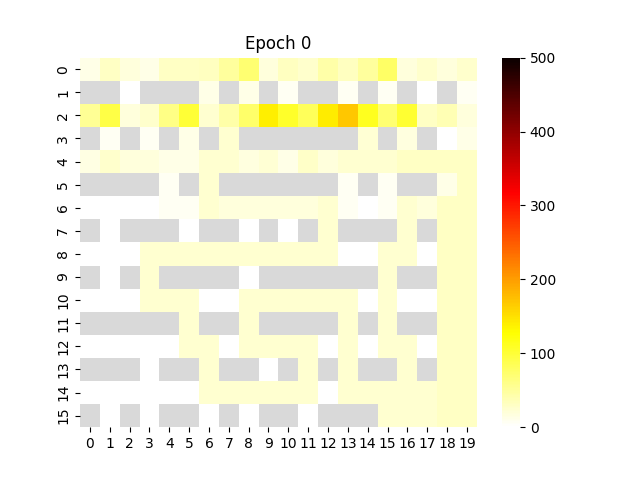
\includegraphics[width=0.9\linewidth]{figs/heatmap_static.png}
        \caption{Static compiler}
    \end{subfigure}
    \begin{subfigure}{\columnwidth}
        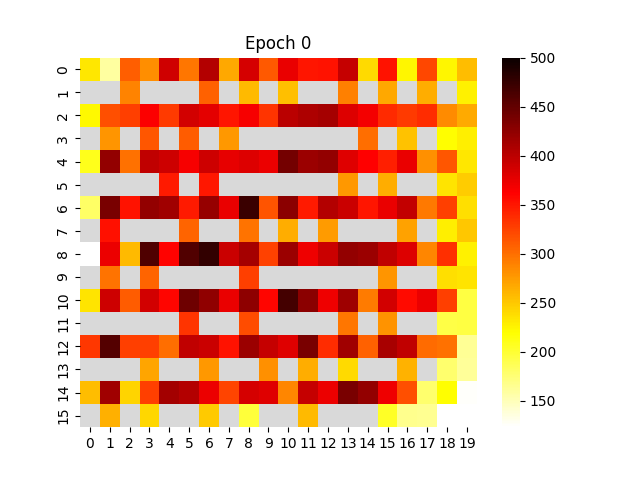
\includegraphics[width=0.9\linewidth]{figs/heatmap_dynamic.png}
        \caption{Dynamic compiler ($k = 25$)}
    \end{subfigure}
    \caption{Heatmap of the ancilla qubits for different compilers for the first $1000$ cycles for the QV\_n100 benchmark (the greyed blocks are the data qubits)}
    \label{fig:heatmap}
\end{figure}

We randomly generated a 2D grid with $50\%$ probability of the data qubit being a compact or compressed patch. For the static compiler, the compilation was done before the execution. For the dynamic compiler, compilation was done on-the-fly and the compiler was run for different parameters. We used the QASM Benchmarks from \cite{li2022qasmbench} by choosing circuits with significant number of Rz gates. We transpiled these benchmarks on Qiskit\cite{Qiskit} to the basis gate set of $X, H, Rz, CNOT$ at an optimization level of $2$ and then simulated the execution of the assembled circuits. We tested the circuit with different values of $k$. For the case of $k = 0$, i.e., where we compute the MST for each CNOT operation, we introduced stalls during the execution of the circuit. For all the executions, we assume $p$ (number of cycles it takes to compute the MST) to be $100$. Figure~\ref{fig:plot} contains the plot of execution times for physical qubit error rate $10^{-3}$ and a code distance of $7$.\par
We observe a significant improvement in the execution times for the case of dynamic compiler, even after accounting for the stalls due to MST computation. The improvement is due to maximum utilization of the ancillas during the preparation phase and minimal waiting time for each gate operation. This can also be observed from the heatmap of the ancillas for the total activity in $1000$ cycles as shown in Figure~\ref{fig:heatmap}. Unlike the static case, the ancillas are active for almost half of the epoch duration. It was also observed that the the performance improvements are maintained as the physical error rates are reduced.

\section{Conclusion}
Fault-tolerant quantum architectures are still far from being realised on physical systems. Various error correction techniques have been proposed, surface codes being one of them. The surface code architecture does not natively support non-Clifford gates and thus require specialized support for such operations. Continuous rotation angle architectures have been proposed that allow for localized, low-latency ancilla preparation in the required states. However, this leads to the problem of supporting dynamic ancilla allocation to minimize runtime. Our work tackles this problem and we propose a dynamic compilation technique that utilizes the variable ancilla availability and activity to perform efficient allocation for different gate operations in parallel, thus minimising the total program execution time. We improve significantly over the basseline proposals while simultaneously minimizing classical overhead for realtime recompilation.
% \par
% The ideas proposed in our work are not only limited to compilation for SARA but can directly be used for compilation for any architecture that involves non-deterministic steps and/or variable availability of ancilla resources.
